\section{Results}
\label{sec:results}

\subsection{RQ1: Audit Signal and Cost}

\begin{figure}[htbp]
\centering
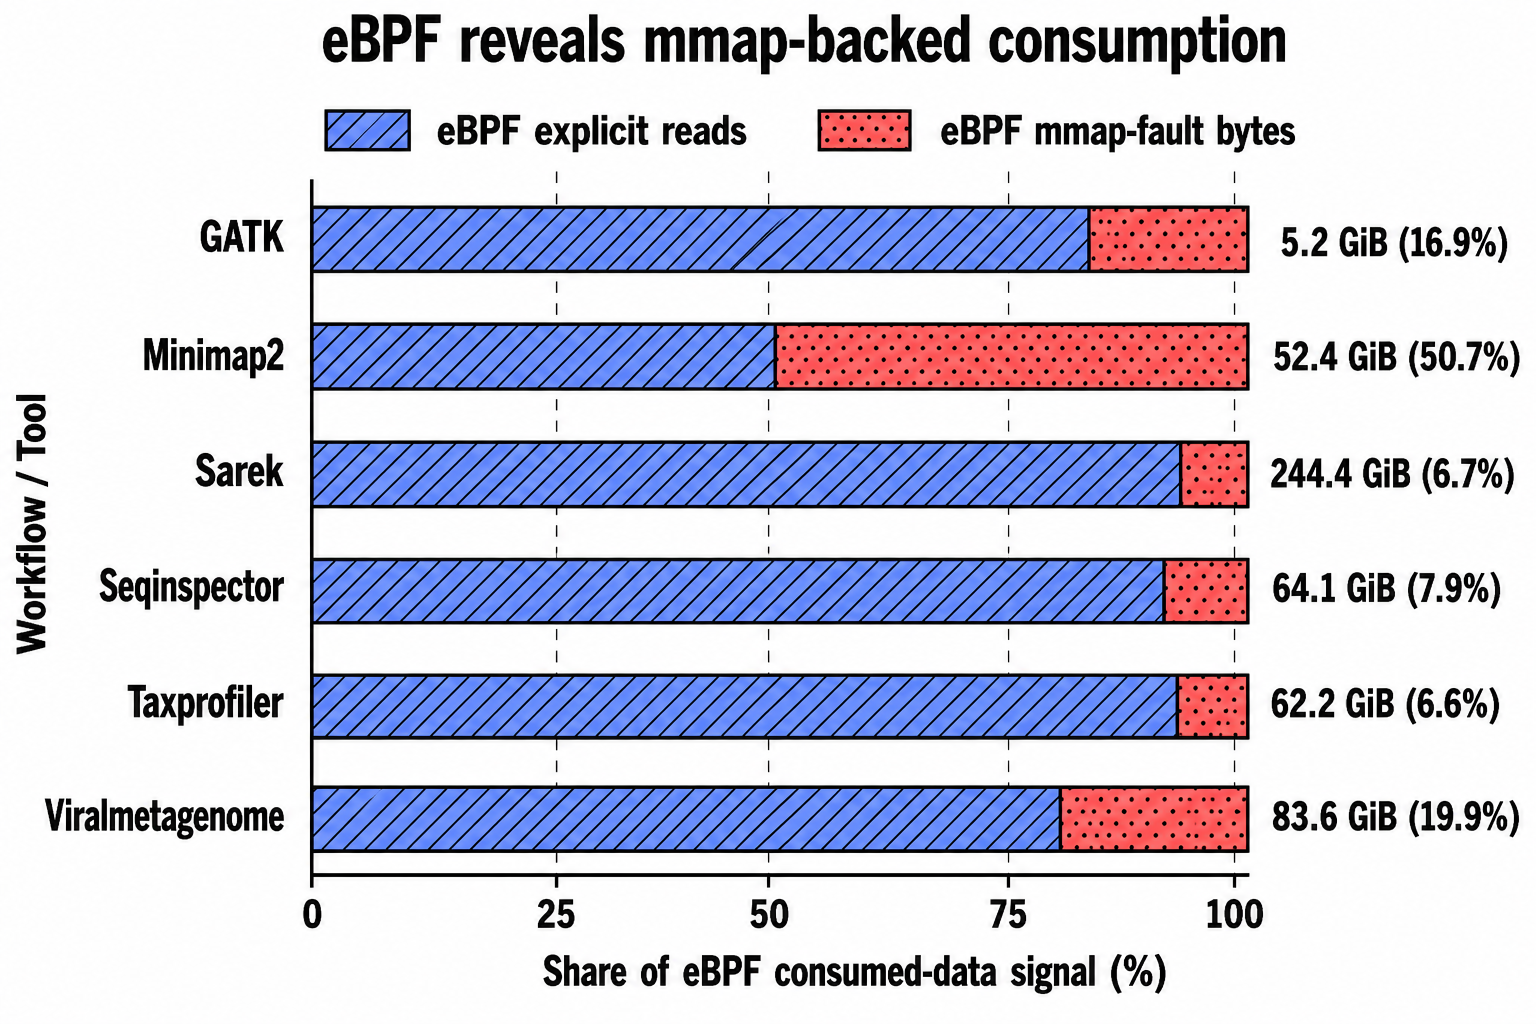
\includegraphics[width=\columnwidth]{source/Figures/fig_rq1_mmap_backed_consumption.png}\par\vspace{3pt}
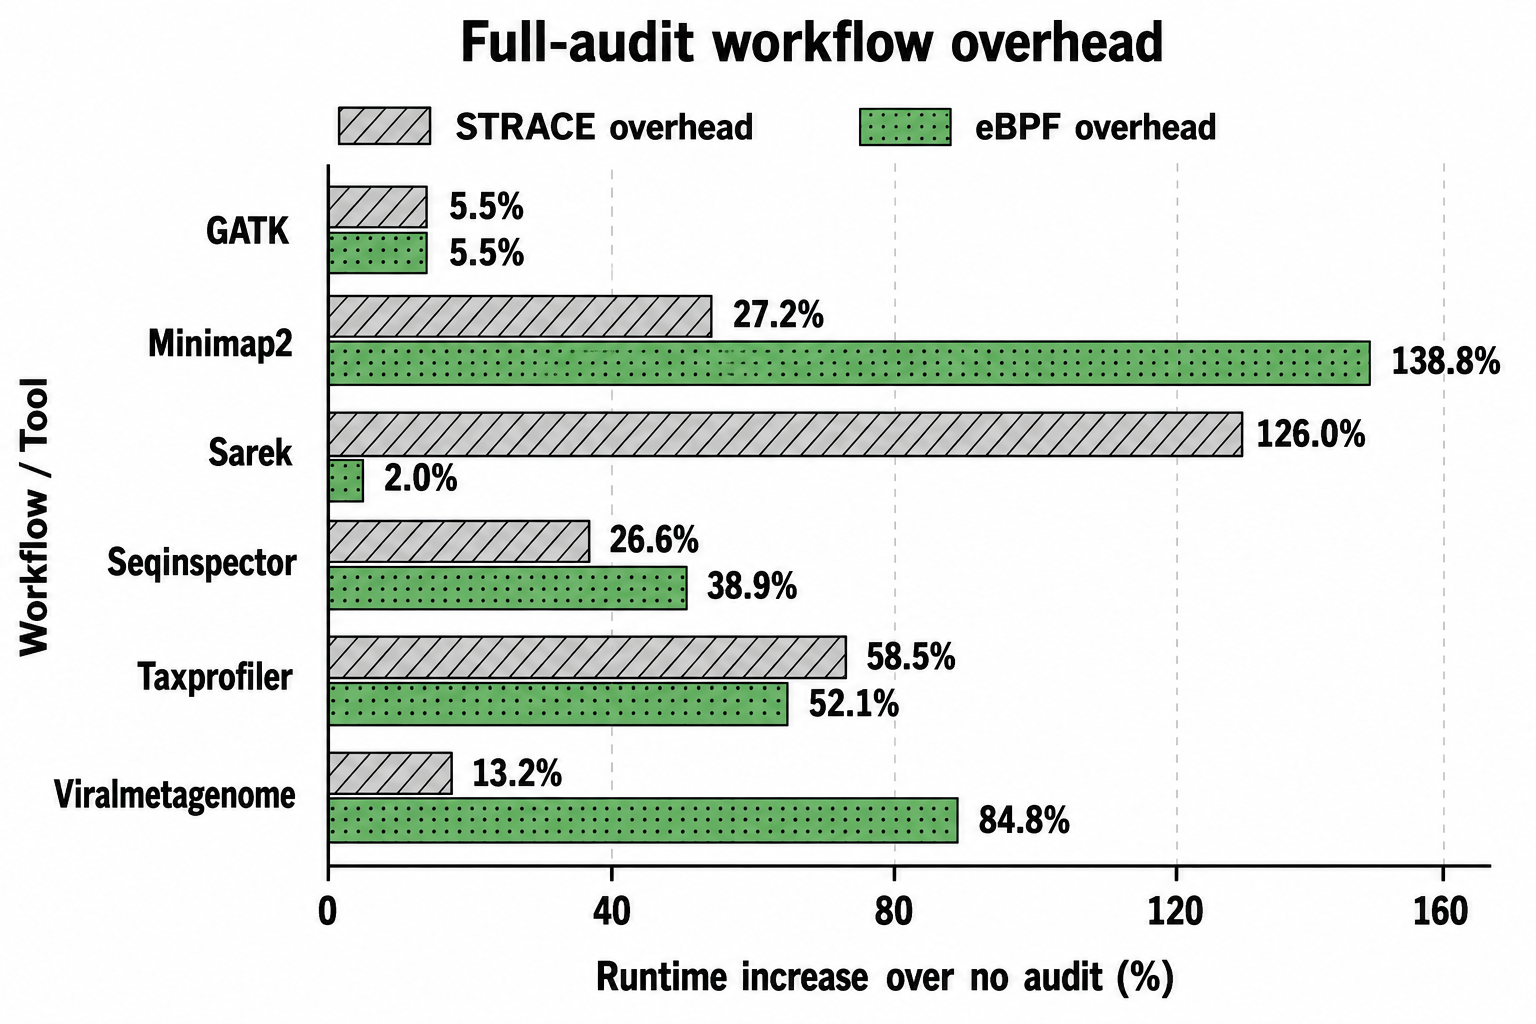
\includegraphics[width=\columnwidth]{source/Figures/fig_rq1_full_audit_workflow_overhead.png}
\caption{RQ1 full auditing. (a) eBPF explicit-read and mmap-fault composition;
labels give mmap bytes and signal share. (b) STRACE and eBPF workflow-runtime
overhead over no audit.}
\label{fig:rq1-consumed}
\end{figure}

Figure~\ref{fig:rq1-consumed}(a) places workflows on the y-axis and the
percentage composition of the eBPF consumed-data signal on the x-axis. 
%Each
% stacked bar separates explicit-read bytes from mmap-fault bytes; labels report
% the absolute mmap-fault volume and its percentage of the total signal.
% Figure~\ref{fig:rq1-consumed}(b) again places workflows on the y-axis, while
% the x-axis reports the end-to-end runtime increase relative to the matched
% no-audit execution. Gray and green bars represent STRACE and eBPF,
% respectively.
As Fig.~\ref{fig:rq1-consumed}(a) shows, mmap faults contribute 50.7\% of
Minimap2's consumed-data signal and 16.9--19.9\% for GATK and
Viralmetagenome, demonstrating that explicit reads alone can miss substantial
consumption. Figure~\ref{fig:rq1-consumed}(b) shows that eBPF full-audit
overhead is not uniformly lower than STRACE: it is similar or lower for GATK,
Sarek, and Taxprofiler, but higher for the other workflows. Thus, eBPF's main
benefit is visibility into mmap-backed consumption, while its variable
full-audit cost motivates selective auditing.

\subsection{RQ2: Consumed-Data Feedback}

\begin{figure*}[!t]
      \centering
      \subfloat[RQ2 underallocations with different splits.]{
          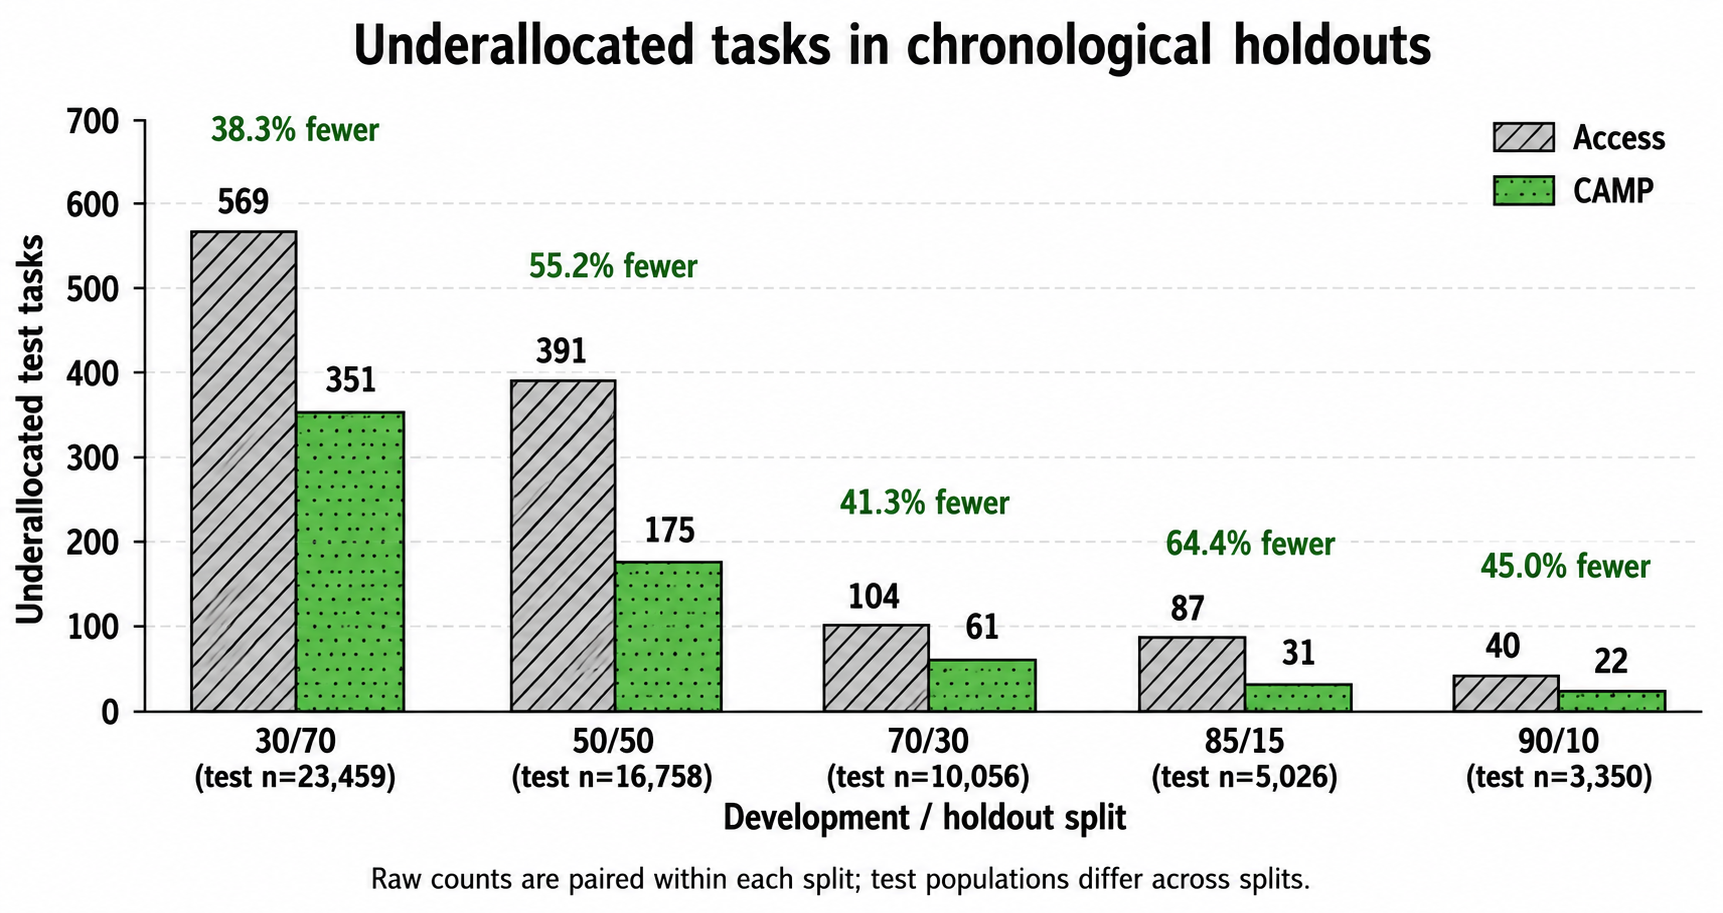
\includegraphics[width=0.48\textwidth]
          {source/Figures/RQ2_Under_allocation.png}
          \label{fig:rq2-underallocation}
      }
      \hfill
      \subfloat[RQ2 allocation variance across repeated
      evaluations.]{
          \includegraphics[width=0.48\textwidth]
          {source/Figures/Variance_Final.png}
          \label{fig:rq2-variance}
      }
      \caption{RQ2 allocation safety and robustness. }
      \label{fig:rq2-combined}
  \end{figure*}

Figure~\ref{fig:rq2-combined}\subref{fig:rq2-underallocation} places the
chronological development/holdout split on the x-axis and the raw number of
underallocated held-out tasks on the y-axis.
%Gray and green bars represent Access and CAMP,
%respectively. 
Figure~\ref{fig:rq2-combined}\subref{fig:rq2-variance} uses the same x-axis and
reports \toolname{} underallocations per
1,000 held-out tasks on the y-axis. The five training seeds are shown as
colored points; diamonds and error bars report the five-seed mean and 95\%
confidence interval, while CV is the coefficient of variation.

As Fig.~\ref{fig:rq2-combined}\subref{fig:rq2-underallocation} shows,
\toolname{} underallocates fewer tasks at all five splits, with reductions of
38.3\%, 55.2\%, 41.3\%, 64.4\%, and 45.0\%, respectively. Panel (b) shows that
85/15 has the greatest seed variation (CV 67.4\%), whereas 70/30 has the lowest
variation (CV 5.9\%). In the primary 85/15 run (seed 1996), \toolname{} reduces
underallocations by 64.37\% and unused memory-time by 37.18\%, while increasing
total requested memory by 31.50\%. Thus, consumed-data feedback reduces
underallocations across the displayed chronological splits, while seed
sensitivity varies across splits.
% \subsection{RQ3: Live Cold-to-Warm Feedback}

% \begin{figure*}[!t]
% \centering
% \includegraphics[width=0.96\textwidth]{source/Figures/fig_rq4_bowtie_feedback.png}
% \caption{RQ3 live 6,000-task Bowtie2 cold and fresh warm runs: (a) observed
% peak and CAMP request; (b) unused memory-time; (c) first-attempt allocation
% margin relative to observed peak.}
% \label{fig:rq3-live}
% \end{figure*}

% Figure~\ref{fig:rq3-live}(a) places the cold and warm runs on the x-axis and
% aggregate memory in GiB on the y-axis. Gray and green bars represent observed
% peak memory and the CAMP request, respectively. Panel (b) uses the same x-axis
% and reports runtime-weighted unused memory in GiB-hours on a logarithmic
% y-axis. Panel (c) places the percentage of tasks on the y-axis and divides each
% run according to how far its first memory request was above or below observed
% peak RSS.

% As Fig.~\ref{fig:rq3-live}(a) shows, nearly identical aggregate peaks
% (238.50/238.82~GiB) accompany a 71.96\% request reduction, from 898.39 to
% 251.93~GiB. Panel (b) shows unused memory-time falling from 23.95 to
% 0.018~GiB-hours, while panel (c) shows tasks requested more than 25\% above
% peak falling from 16.73\% to 0.27\%. Both executions finish with zero
% OOM-classified exits and 99.93/99.78\% first-attempt coverage. Thus, persisted
% feedback removes most cold-start reservation cost while maintaining high
% coverage.

\subsection{RQ:3 External Comparison with Sizey}

\begin{figure}[!t]
\centering
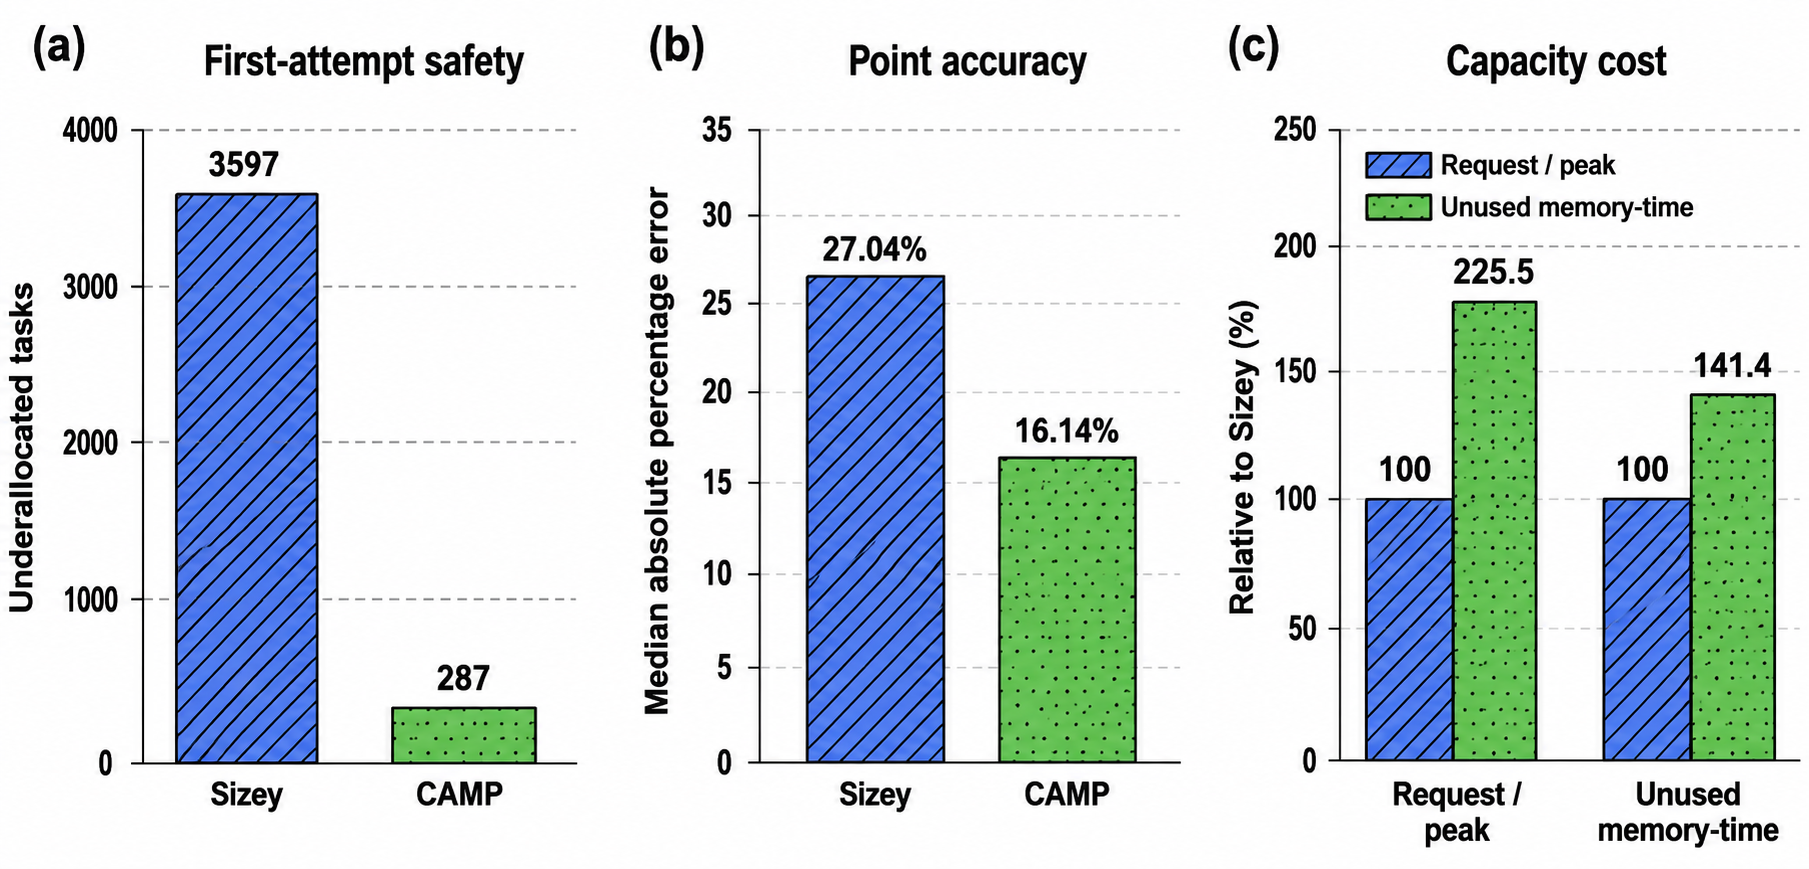
\includegraphics[width=\columnwidth]{source/Figures/fig_sizey_vs_camp.png}
\caption{ 21,337-task comparison with Sizey:
(a) underallocations; (b) median absolute percentage error; (c) request/peak
and unused memory-time normalized to Sizey.}
\label{fig:sizey-comparison}
\end{figure}

Figure~\ref{fig:sizey-comparison}(a) places Sizey and \toolname{} on the x-axis and
the number of underallocated tasks on the y-axis. Panel (b) uses the same
x-axis and reports median absolute percentage error on the y-axis. Panel (c)
places request-to-peak ratio and unused memory-time on the x-axis and reports
each value relative to Sizey on the y-axis; Sizey is normalized to 100\%.

As Fig.~\ref{fig:sizey-comparison}(a) shows, \toolname reduces underallocations
from 3,597 to 287, a 92.02\% reduction, and raises first-attempt coverage from
83.14\% to 98.65\%. Panel (b) shows median absolute percentage error falling
from 27.04\% to 16.14\%, a 40.31\% improvement. Panel (c) shows the capacity
tradeoff: \toolname{}'s request-to-peak ratio is 225.5\% of Sizey's and its unused
memory-time is 141.4\%. Thus, \toolname substantially improves safety and point
accuracy, but uses more reserved capacity than Sizey.

\subsection{RQ:4 Selective Auditing}

\begin{figure}[!t]
\centering
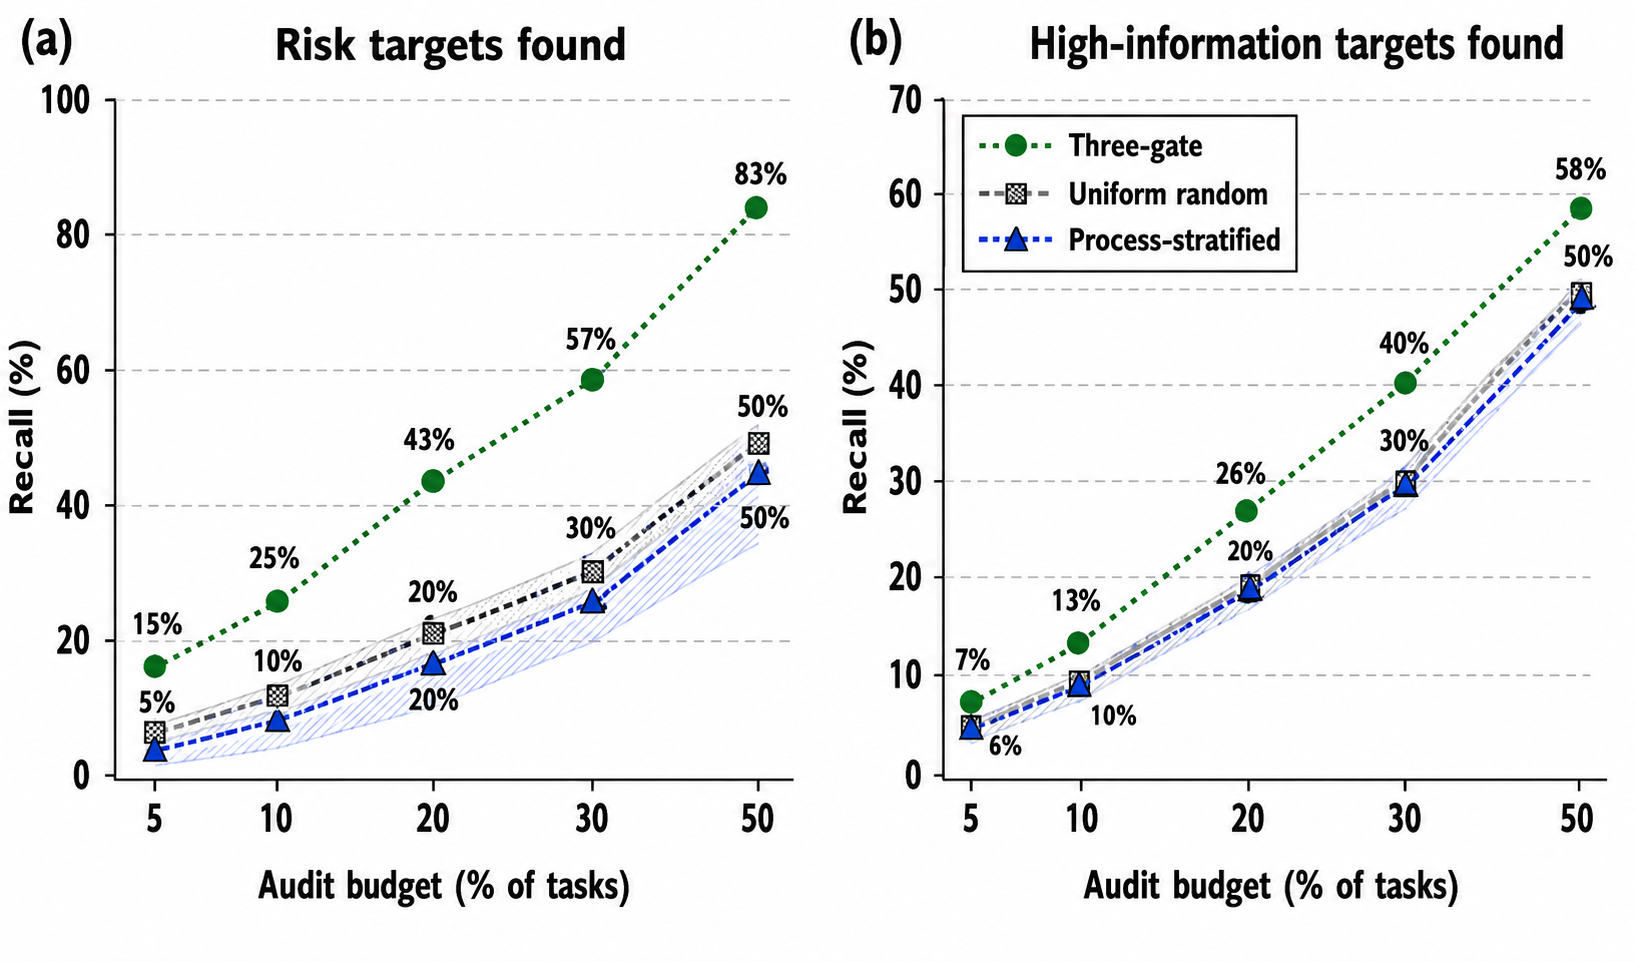
\includegraphics[width=\columnwidth]{source/Figures/fig_rq3_selective_audit.png}
\caption{ RQ4 equal-count selective-audit recall. Curves are means over 1,000
repetitions; shading gives empirical 95\% random-baseline intervals and the
dotted diagonal is budget-proportional recall.}
\label{fig:rq3-auditing}
\end{figure}

Figure~\ref{fig:rq3-auditing} places the audit budget, expressed as the
percentage of tasks audited, on the x-axis and target recall on the y-axis.
Panel (a) reports recall of risk targets whose active memory request would be
smaller than peak RSS. Panel (b) reports recall of high-information targets
meeting the joint memory-tail and consumption-utility label defined by the
heavy-information gate. All policies select the same number of tasks at each
budget.

In Fig.~\ref{fig:rq3-auditing}(a), \toolname recalls 15\%, 25\%, 43\%, 57\%, and
83\% of risk targets at 5\%, 10\%, 20\%, 30\%, and 50\% budgets, respectively,
compared with 5\%, 10\%, 20\%, 30\%, and 50\% for uniform random selection.
Panel (b) shows high-information recall of 7\%, 13\%, 26\%, 40\%, and 58\%,
again above both equal-count random baselines at every displayed budget. Thus,
the gates concentrate audits most strongly on underallocation risk while also
finding more tasks useful for refreshing consumption-aware models.

\subsection{RQ5: Live Cold-to-Warm Feedback}

\begin{figure*}[!t]
\centering
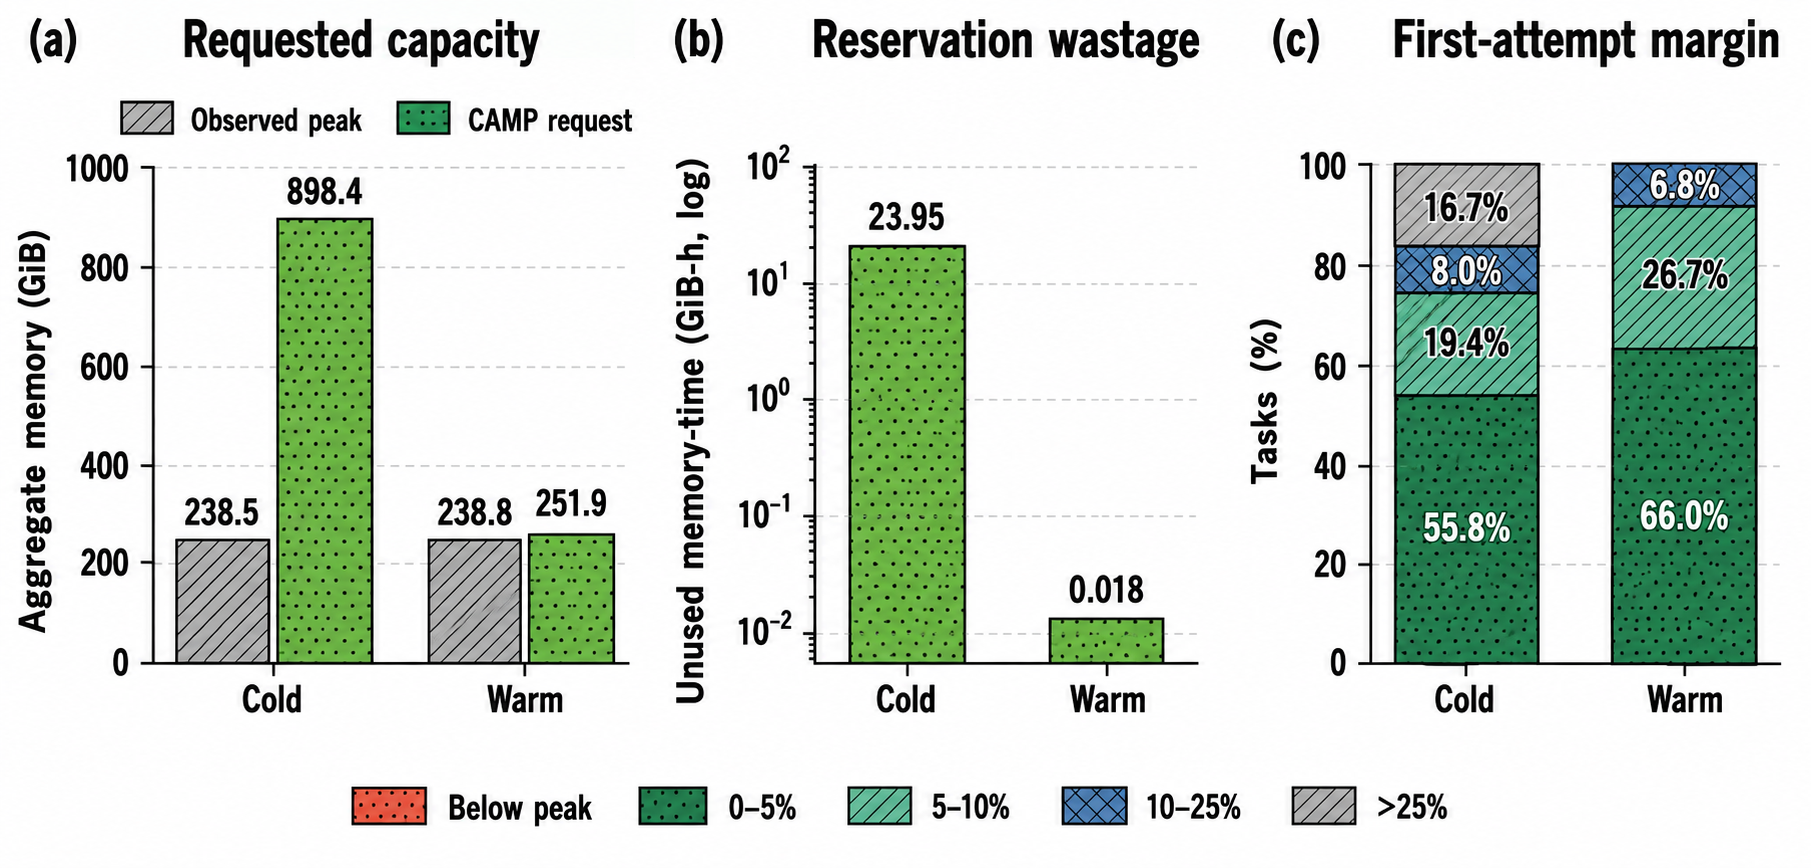
\includegraphics[width=0.96\textwidth]{source/Figures/RQ_5_Bowtie_Cold_And_Warm_LiveRun.png}
\caption{RQ5 live 6,000-task Bowtie2 cold and fresh warm runs: (a) aggregate
observed peak and first-requested memory; (b) runtime-weighted unused
memory-time; and (c) first-attempt allocation margin relative to observed peak
RSS.}
\label{fig:rq5-live}
\end{figure*}

Figure~\ref{fig:rq5-live}(a) compares aggregate observed peak memory with the
memory requested before each task outcome was known. The cold and warm runs
execute 6,000 logical Bowtie2 tasks each and have nearly identical aggregate
observed peaks: 238.50 and 238.82~GiB, respectively. In contrast, aggregate
first-requested memory falls from 898.39~GiB in the cold run to 251.93~GiB in
the warm run, a 71.96\% reduction. The warm request is only about 5.5\% above
aggregate observed demand, whereas the cold request is approximately 3.77
times the observed peak.

Panel (b) weights excess requested memory by task runtime. Unused memory-time
falls from 23.954~GiB-hours to 0.018~GiB-hours, a 99.93\% reduction. This
three-order-of-magnitude decrease shows that feedback from the completed cold
run removes most of the reservation cost for the subsequent fresh execution,
without relying on workflow-cache reuse.

Panel (c) explains the change at task granularity. The share of tasks requested
within 10\% above their observed peak rises from 75.25\% to 92.73\%, while the
share requested more than 25\% above peak falls from 16.73\% to 0.27\%. The
tighter warm allocations introduce a small safety tradeoff: first requests
below observed peak increase from 4 to 13 tasks because the warm run makes tighter memory requests, leaving less buffer for prediction error, so first-attempt coverage
changes from 99.93\% to 99.78\%. Overall, the cold-to-warm experiment demonstrates that completed Bowtie2
outcomes can substantially tighten later memory reservations while retaining
very high first-attempt coverage.
